\documentclass{article}

\usepackage{fancyhdr}
\usepackage{extramarks}
\usepackage{amsmath}
\usepackage{amsthm}
\usepackage{amsfonts}
\usepackage{tikz}
\usepackage[plain]{algorithm}
\usepackage{algpseudocode}

\usepackage{verbatim}
\usepackage{graphicx}
\graphicspath{ {images/} }

\usetikzlibrary{automata,positioning}

%
% Basic Document Settings
%

\topmargin=-0.45in
\evensidemargin=0in
\oddsidemargin=0in
\textwidth=6.5in
\textheight=9.0in
\headsep=0.25in

\linespread{1.1}

\pagestyle{fancy}
\lhead{\hmwkAuthorName}
\chead{\hmwkClass\ : \hmwkTitle} %(\hmwkClassInstructor\) \hmwkClassTime): 
\rhead{\firstxmark}
\lfoot{\lastxmark}
\cfoot{\thepage}

\renewcommand\headrulewidth{0.4pt}
\renewcommand\footrulewidth{0.4pt}

\setlength\parindent{0pt}

%
% Create Problem Sections
%

\newcommand{\enterProblemHeader}[1]{
    \nobreak\extramarks{}{Problem (\alph{#1}) continued on next page\ldots}\nobreak{}
    \nobreak\extramarks{Problem (\alph{#1}) (continued)}{Problem (\alph{#1}) continued on next page\ldots}\nobreak{}
}

\newcommand{\exitProblemHeader}[1]{
    \nobreak\extramarks{Problem (\alph{#1}) (continued)}{Problem (\alph{#1}) continued on next page\ldots}\nobreak{}
    \stepcounter{#1}
    \nobreak\extramarks{Problem (\alph{#1})}{}\nobreak{}
}

\setcounter{secnumdepth}{0}
\newcounter{partCounter}
\newcounter{homeworkProblemCounter}
\setcounter{homeworkProblemCounter}{1}
\nobreak\extramarks{Problem (\alph{homeworkProblemCounter})}{}\nobreak{}

%
% Homework Problem Environment
%
% This environment takes an optional argument. When given, it will adjust the
% problem counter. This is useful for when the problems given for your
% assignment aren't sequential. See the last 3 problems of this template for an
% example.
%
\newenvironment{homeworkProblem}[1][-1]{
    \ifnum#1>0
        \setcounter{homeworkProblemCounter}{#1}
    \fi
    \section{Problem (\alph{homeworkProblemCounter})}
    \setcounter{partCounter}{1}
    \enterProblemHeader{homeworkProblemCounter}
}{
    \exitProblemHeader{homeworkProblemCounter}
}

%
% Homework Details
%   - Title
%   - Due date
%   - Class
%   - Section/Time
%   - Instructor
%   - Author
%

\newcommand{\hmwkTitle}{Test Exercise\ \#1}
%\newcommand{\hmwkDueDate}{February 12, 2014}
\newcommand{\hmwkClass}{MOOC Econometrics}
%\newcommand{\hmwkClassTime}{Section A}
%\newcommand{\hmwkClassInstructor}{Professor Isaac Newton}
\newcommand{\hmwkAuthorName}{\textbf{Greg Faletto}} % \and \textbf{Davis Josh}}

%
% Title Page
%

\title{
    \vspace{2in}
    \textmd{\textbf{\hmwkClass:\ \hmwkTitle}}\\
    %\normalsize\vspace{0.1in}\small{Due\ on\ \hmwkDueDate\ at 3:10pm}\\
    %\vspace{0.1in}\large{\textit{\hmwkClassInstructor\ \hmwkClassTime}}
    \vspace{3in}
}

\author{\hmwkAuthorName}
\date{}

\renewcommand{\part}[1]{\textbf{\large Part \Alph{partCounter}}\stepcounter{partCounter}\\}

%
% Various Helper Commands
%

% Useful for algorithms
\newcommand{\alg}[1]{\textsc{\bfseries \footnotesize #1}}

% For derivatives
\newcommand{\deriv}[1]{\frac{\mathrm{d}}{\mathrm{d}x} (#1)}

% For partial derivatives
\newcommand{\pderiv}[2]{\frac{\partial}{\partial #1} (#2)}

% Integral dx
\newcommand{\dx}{\mathrm{d}x}

% Alias for the Solution section header
\newcommand{\solution}{\textbf{\large Solution}}

% Probability commands: Expectation, Variance, Covariance, Bias
\newcommand{\E}{\mathrm{E}}
\newcommand{\Var}{\mathrm{Var}}
\newcommand{\Cov}{\mathrm{Cov}}
\newcommand{\Bias}{\mathrm{Bias}}

\begin{document}

\maketitle

\pagebreak

\section{Questions}

This exercise considers an example of data that do not satisfy all the standard assumptions of simple regression. In the considered case, assumption A6 that the coefficients \(\alpha\) and \(\beta\) are the same for all observations is violated. The dataset contains survey outcomes of a travel agency that wishes to improve recommendation strategies for its clients. The dataset contains 26 observations on age and average daily expenditures during holidays.

\begin{homeworkProblem}

Use all data to estimate the coefficients \(a\) and \(b\) in a simple regression model, where expenditures is the dependent variable and age is the explanatory factor. Also compute the standard error and the \(t\)-value of \(b\).
\\

    \solution
  
  % \verbatiminput{Acode.txt}
   
    \verbatiminput{AOutput2.txt}
    
\end{homeworkProblem}

\pagebreak

\begin{homeworkProblem}
    Make the scatter diagram of expenditures against age and add the regression line \(y = a + bx\) of part (a) in this diagram. What conclusion do you draw from this diagram?   
\\

    \solution
    \\
    
    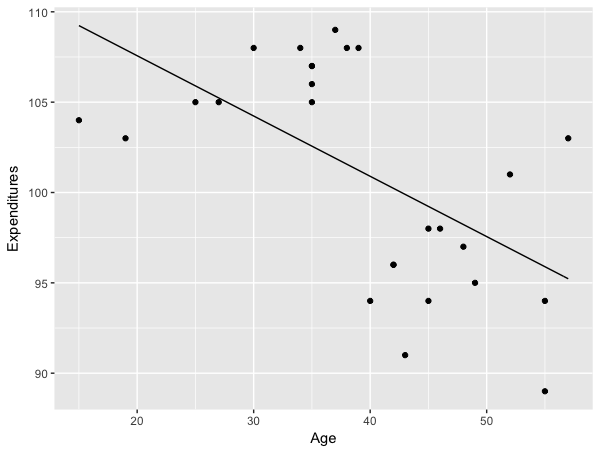
\includegraphics[scale=0.75]{b}
    
    The conclusion I draw from this diagram is that Age provides some predictive value in predicting Expenditures, but it seems as though people under 40 have significantly different spending habits as a function of age than people over 40. Specifically, for people under 40 expenditures seem to increase with age, and for people over 40 there isn't a clear trend. Splitting the data into two groups might yield better results.    

\end{homeworkProblem}

\pagebreak

\begin{homeworkProblem}

It seems there are two sets of observations in the scatter diagram, one for clients aged 40 or higher and another for clients aged below 40. Divide the sample into these two clusters, and for each cluster estimate the coefficients \(a\) and \(b\) and determine the standard error and \(t\)-value of \(b\).
\\

    \solution
  \verbatiminput{c.txt}
  
\end{homeworkProblem}
  
\begin{homeworkProblem}
  
  Discuss and explain the main differences between the outcomes in parts (a) and (c). Describe in words what you have learned from these results.
  \\
  
  \solution
  \\
  
  In part (c), I found a significantly different way to model the data by splitting the data into two groups and modeling them separately. Based on our limited sample data set, this seems to provide more predictive value than simply grouping all the data together and making one model. We may need a larger sample before we can know for sure if this is the best model for the data. Sometimes it may be better to group the data into different groups and then model the data separately.
  \\
  
  The \(95\%\) confidence interval for b includes \(0\) in the model for customers 40 and over. This means we do not have significant evidence to reject the null hypothesis that \(b = 0\) for customers over 40--in other words, we do not have significant evidence suggesting a correlation between age and expenditures for customers over 40.
  \\
  
  The \(95\%\) confidence interval for b does not \(0\) in the model for customers under 40. This means we have significant evidence to reject the null hypothesis that \(b = 0\) for customers under 40. We have significant evidence suggesting a correlation between age and expenditures for customers over 40.
  
\end{homeworkProblem}

\end{document}
